\documentclass[12pt]{article}
\usepackage{graphicx}
\usepackage{draftwatermark}
\SetWatermarkText{DRAFT}
\SetWatermarkScale{5}

\title{FURST Feed Optic Specification}
\date{Version 0.2, 2017-Jul-10}
\author{C.\ Kankelborg}

\begin{document}
\maketitle

\section{Introduction}

The Full-sun Ultraviolet Rocket SpecTrometer (FURST) is a \emph{proposed} NASA sounding rocket mission to obtain well calibrated FUV spectra of the full sun from 120-200\,nm. This document describes the FURST feed optics. These are small glass cylinders, to be coated by the customer, which reflect sunlight into the spectrometer. \emph{We are presently requesting a quotation for budgetary purposes, to support the proposal process. Response is requested by July 14.}



\section{Requirements}
Table \ref{tab:spec} lists requirements for the feed optics. Dimensions and layout are specified in figure \ref{fig:cylinder}. 

\begin{figure}
   \begin{center}
      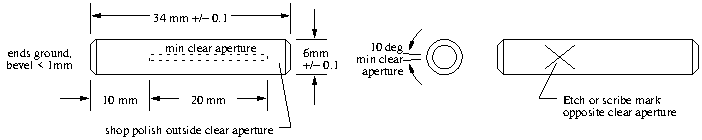
\includegraphics[width=0.95\textheight, angle=90]{cylinder.pdf}
   \end{center}
   \caption{Sketch of the feed optic design.}\label{fig:cylinder}
\end{figure}


\begin{table}
\caption{Requirements Table for the FURST grating. Verification methods are T (test), 
   M (measurement), I (inspection), C (calculation), D (design/mfg process).}\label{tab:spec}
   \small
   \begin{tabular}{llc} \hline
      Specification     & Requirement                                     & Verification \\ \hline
      Type     & Cylindrical mirror per fig \ref{fig:cylinder}            & I \\
      Radius   & $3\pm 0.05$\,mm convex cylinder                          & M \\
      Wavefront error & $\lambda/4$ PV over clear aperture                & M \\
      Material & Pyrex                                                    & mat'l cert \\
      Dimensions & per fig \ref{fig:cylinder}                             & I \\
      Diameter uniformity & $\pm 25\,\mu$m end to end, each part          & I \\
      Microroughness & 3.5\,nm RMS, periods 0.1-10\,$\mu$m on clear aperture & M \\
      Surface quality & 20-10 scratch-dig on clear aperture & I \\ % added 2017-Jul-10
      \hline
   \end{tabular}
   \normalsize
\end{table}





\section{Deliverables} \label{sec:deliverables}
\begin{enumerate}
   \item 25 uncoated feed optics meeting the above specifications (11 flight plus spares).
   \item Conformance report, including all test results relevant to this specification.
\end{enumerate}


\end{document}